\documentclass[a4paper,11pt]{article}
\usepackage[margin=2.4cm]{geometry}
\usepackage{ctex}
\usepackage{amsmath,amssymb}
\usepackage{booktabs}
\usepackage{multirow}
\usepackage{array}
\usepackage{makecell}
\usepackage{siunitx}
\usepackage{xcolor}
\usepackage{hyperref}
\usepackage{enumitem}
\usepackage{float}
\usepackage{graphicx}

\hypersetup{colorlinks=true, linkcolor=blue!60!black, citecolor=blue!60!black, urlcolor=blue!60!black}

\title{\textbf{NN proton 重建主模型评估 —— 在 ypol elastic\_allair 上与 RK 对比}}
\author{Baiting Tian \\ RIKEN 仁科中心 / DPOL 实验}
\date{2026 年 5 月 3 日}

\begin{document}
\maketitle

\section*{摘要}
对当前 PDC$\to$target proton 动量 NN 主模型 (\texttt{formal\_B115T3deg/20260420\_184345}) 在
\texttt{ypol\_new\_20260413\_elastic\_allair} 全 16 cell (Sn112/Sn124 $\times$ g050/g060/g070/g080 $\times$ ynp/ypn,
每 cell 10\,000 事件) g4output 上做 forward 推理, 并与同输入的 RK 重建 (\texttt{ypol\_phys\_20260428\_zh.tex} 报告所用 \texttt{fixed-target-pdc-only} 模式) 做\textbf{逐事件}残差对比。
主要结论:
\begin{itemize}[nosep]
    \item NN 在所有事件上都给出输出 (100\% 通过率), RK 通过率 98.93\% (\texttt{n\_reco\_proton}>0).
    \item \textbf{核心 1$\sigma$}: RK 略胜 NN —— $\Delta p_x$ 半宽 5.86 vs 6.01, $\Delta p_y$ 1.52 vs 1.37 (NN 反而更窄), $\Delta p_z$ 5.88 vs 6.25 MeV/$c$.
    \item \textbf{尾部}: NN 完胜 RK —— $|\vec p|$ RMSE 10.8 vs 39.9 MeV/$c$, $\Delta p_z$ RMSE 13.4 vs 46.4 MeV/$c$. RK 在 $\sim$2\% 事件上有数百 MeV 的灾难性失败 (RK 报告 §1.3 提到的 dE/dx + 线性化失效), NN 没有这种失败模式.
    \item NN 引入轻微的系统偏: $|\vec p|$ med = $+1.6$ MeV/$c$, RK 是 $-1.0$ MeV/$c$; NN $\Delta p_y$ 有 $+0.5$ MeV/$c$ 的偏, RK 几乎为 0.
    \item 训练域 ($p_T\le 100$ MeV/$c$, $p_z\in[560,680]$) 与本测试样本几乎完全覆盖 (97\% 与 99.5\%), 域外性能未在本报告评估.
\end{itemize}

\section{1. 主模型简介}

\subsection{1.1 模型与 artifact}
\begin{itemize}[nosep]
    \item 路径: \texttt{data/nn\_target\_momentum/formal\_B115T3deg/20260420\_184345/}
    \item 4 件套: \texttt{model.pt} (107 KB) + \texttt{model\_meta.json} + \texttt{model\_cpp.json} (765 KB) + \texttt{training\_history.csv}
    \item C++ 推理由 \texttt{libs/analysis\_pdc\_reco/src/PDCNNMomentumReconstructor.cc} 加载 \texttt{model\_cpp.json}, 在 \texttt{reconstruct\_target\_momentum --backend nn} 中调用.
\end{itemize}

\subsection{1.2 网络结构}
固定 6$\to$3 MLP, 隐藏层全 ReLU:
\[
    \mathbb{R}^6 \xrightarrow{\text{Linear+ReLU}} \mathbb{R}^{128}
    \xrightarrow{\text{Linear+ReLU}} \mathbb{R}^{128}
    \xrightarrow{\text{Linear+ReLU}} \mathbb{R}^{64}
    \xrightarrow{\text{Linear}} \mathbb{R}^{3}
\]
\textbf{输入特征 (6 维)}: $(\,x, y, z\,)_\text{PDC1}$ 和 $(\,x, y, z\,)_\text{PDC2}$ —— 即 PDC1, PDC2 两层 drift chamber 的击中点 (lab frame, mm).
PDC 击中前在 \texttt{build\_dataset.C} 内加 $\sigma_u = \sigma_v = 0.5$ mm 的高斯位置噪声以匹配运行时分辨。
\textbf{输出 (3 维)}: target 处真值 proton 动量 $(p_x, p_y, p_z)$ (MeV/$c$, target frame).
输入用训练集自身的 \texttt{x\_mean / x\_std} 做 z-score, 输出未做归一化。

\subsection{1.3 训练数据集}

数据由 \texttt{run\_formal\_training.sh} 生成, 三套\textbf{独立种子}的 Geant4 仿真 + \texttt{build\_dataset.C} 提取:

\begin{table}[H]
\centering\footnotesize
\caption{主模型训练 / 验证 / 测试集 (来自 \texttt{manifest.json}, campaign \texttt{formal\_B115T3deg\_diskR150\_pz500\_700} 但实际 manifest 抽样为 R=100, $p_z\in[560,680]$)}
\begin{tabular}{lrrr}
\toprule
split & requested events & seed & dataset rows (kept) \\
\midrule
train & 200\,000 & 20260301 & 93\,970 \\
val   & 30\,000  & 20260302 & 14\,024 \\
test  & 30\,000  & 20260303 & 14\,087 \\
\bottomrule
\end{tabular}
\end{table}

\textbf{动量采样}:
\begin{itemize}[nosep]
    \item $(p_x, p_y)$: 在半径 $R = 100$ MeV/$c$ 的二维圆盘内均匀,
    \item $p_z$: 在 $[560, 680]$ MeV/$c$ 区间均匀.
\end{itemize}
\textbf{几何}: \texttt{configs/simulation/DbeamTest/detailMag1to1.2T/geometry\_B115T\_pdcOptimized\_20260227\_target3deg.mac}
(SHA-256 \texttt{52006d...e244e}), 靶倾角 $3°$, 靶位置 $(-12.49, 0.009, -1069.46)$ mm.

\subsection{1.4 训练超参数}

\begin{table}[H]
\centering\footnotesize
\begin{tabular}{ll}
\toprule
项目 & 设置 \\
\midrule
optimizer        & Adam, lr=$1\!\times\!10^{-3}$, weight\_decay=$10^{-5}$ \\
batch size       & 1024 \\
loss             & MSELoss (无加权) \\
target normalize & none (直接对 MeV/$c$ 拟合) \\
epochs requested & 120 (best @ epoch 118, 全部 120 跑完) \\
early-stop patience & 12 (未触发) \\
seed             & 20260227 \\
\bottomrule
\end{tabular}
\end{table}

\subsection{1.5 训练时自检指标}
\texttt{model\_meta.json} 自带的 val / test 指标 (单位 MeV/$c$, 在训练分布上, 即 $R\le 100$ disk, $p_z\in[560,680]$):

\begin{table}[H]
\centering\footnotesize
\begin{tabular}{lcccccccc}
\toprule
        & \multicolumn{4}{c}{val (14\,024)}     & \multicolumn{4}{c}{test (14\,087)} \\
\cmidrule(lr){2-5}\cmidrule(lr){6-9}
        & MAE & RMSE & bias & $p_{95}|.|$       & MAE & RMSE & bias & $p_{95}|.|$ \\
\midrule
$p_x$   & 4.28 & 6.70 & $+0.20$ & 10.72         & 4.28 & 6.44 & $+0.16$ & 10.55 \\
$p_y$   & 1.25 & 2.40 & $+0.35$ &  2.98         & 1.24 & 2.45 & $+0.40$ &  2.98 \\
$p_z$   & 3.76 & 5.80 & $-0.35$ &  9.16         & 3.77 & 5.77 & $-0.37$ &  9.27 \\
$|\vec p|$ & 3.93 & 6.08 & $-0.39$ & 9.61       & 3.94 & 6.00 & $-0.41$ &  9.65 \\
\bottomrule
\end{tabular}
\end{table}
\textbf{注意}: best val MSE = 28.08 (=约 5.3 MeV/$c$ RMS), 训练接近收敛但仍有改进空间.

\section{2. 评估方案}

\subsection{2.1 测试样本}
直接复用 RK 报告 (\texttt{ypol\_phys\_20260428\_zh.tex}) 的 16 cell sampled 输入:
\[
    \texttt{build/test\_output/ypol\_phys\_20260428/sampled/<target>\_<gamma><hel>.root}
\]
覆盖 Sn112E190 / Sn124E190 $\times$ g050 / g060 / g070 / g080 $\times$ ynp / ypn, 每 cell 10\,000 事件 (\texttt{subsample\_dbreak.py} 抽样, 同时要求 OK\_PDC1 \& OK\_PDC2), 共 \textbf{160\,000 事件}.

\subsection{2.2 NN 推理命令}
对每个 sampled root 各跑一遍, 全 16 cell 6 路并行约 1 分钟:
\begin{verbatim}
build/bin/reconstruct_target_momentum \
  --input-file  sampled/<tag>.root \
  --output-file reco_nn/<tag>_reco_nn.root \
  --geometry-macro configs/.../geometry_B115T_pdcOptimized_20260227_target3deg.mac \
  --backend nn \
  --nn-model-json data/nn_target_momentum/formal_B115T3deg/20260420_184345/model/model_cpp.json
\end{verbatim}

\subsection{2.3 RK 输出}
来自 \texttt{ypol\_phys\_20260428\_zh.tex} 已有 reco artifact (\texttt{reco/<tag>\_reco.root}), 模式 \texttt{fixed-target-pdc-only}.

\subsection{2.4 抽取与残差定义}
\texttt{scripts/analysis/ypol\_phys/extract\_proton\_rk\_nn.C} 同时打开 RK 与 NN 两棵 \texttt{recoTree}, 按 event\_index 对齐, 抽出每事件:
\[
    (\,\text{truth\_proton\_p4}\,,\;\text{rk\_proton\_p[0]}\,,\;\text{nn\_proton\_p[0]}\,)
\]
到一行 CSV; 每 cell 一份 CSV.
分析脚本 \texttt{analyze\_nn\_vs\_rk\_residuals.py} pool 全 16 cell, 并对两个方法都\textbf{要求 status==0 且 reco $|\vec p|>0$}, 取交集 (apples-to-apples 子集) 计算残差
$\Delta p_i = p_i^\text{reco} - p_i^\text{truth}$, $i \in \{x, y, z\}$ 以及 $\Delta|\vec p| = |\vec p^\text{reco}| - |\vec p^\text{truth}|$.

\subsection{2.5 通过率}
\begin{table}[H]
\centering\footnotesize
\begin{tabular}{lr}
\toprule
项目 & 计数 \\
\midrule
total events read              & 160\,000 \\
truth\_has\_proton             & 160\,000 (100\%) \\
RK 重建成功 (status==0)        & 158\,293 (98.93\%) \\
NN 重建成功 (status==0)        & 160\,000 (100\%) \\
both OK (后续残差子集)         & 158\,293 \\
\bottomrule
\end{tabular}
\end{table}
\textbf{读法}: NN 是纯 forward, 只要 PDC1+PDC2 有击中点就给出输出 (本样本 100\% 满足); RK 在 $\sim$1.1\% 事件上不收敛.

\subsection{2.6 训练域 vs 测试域}
\begin{table}[H]
\centering\footnotesize
\begin{tabular}{lcc}
\toprule
                                 & 训练域           & 本测试样本 truth \\
\midrule
$p_T = \sqrt{p_x^2+p_y^2}$       & uniform disk $\le 100$ MeV/$c$  & median 21.4, $p_{95}=73$, max 351.8 \\
$p_z$                            & uniform $[560, 680]$ MeV/$c$    & median 629.2, 90\% 区间 [621.4, 632.4] \\
样本落在训练域内的比例           & ---                              & $p_T\le100$: 97.1\%, $p_z\in[560,680]$: 99.5\% \\
\bottomrule
\end{tabular}
\end{table}
ypol elastic 是\textbf{近弹性}事件, $\vec p$ 集中在 $|\vec p|\approx 627$ MeV/$c$ 附近, 几乎完全位于训练分布的内部 —— 本评估\textbf{不能外推到 QMD 端 / breakup 端}的更宽 $p_T$ 分布.

\section{3. 残差结果}

\subsection{3.1 总体残差表 (160k 事件 pool, both-OK 子集)}

\begin{table}[H]
\centering\footnotesize
\caption{Per-component 残差汇总 (单位 MeV/$c$). half-width = $(P_{84.135}-P_{15.865})/2$, 接近 1$\sigma$.
RMSE 含尾部, half-width 不含, 两者背离即说明非高斯尾.}
\begin{tabular}{l|rrrr|rrrr}
\toprule
            & \multicolumn{4}{c|}{\textbf{RK}} & \multicolumn{4}{c}{\textbf{NN (formal\_B115T3deg)}} \\
component   & median & half-width & RMSE & $p_{95}|.|$
            & median & half-width & RMSE & $p_{95}|.|$ \\
\midrule
$\Delta p_x$    & $-0.014$ & 5.856 & 17.077 & 12.66 & $-0.813$ & 6.010 & 11.729 & 13.76 \\
$\Delta p_y$    & $-0.122$ & 1.522 &  1.883 &  3.26 & $+0.518$ & \textbf{1.370} &  1.819 &  3.10 \\
$\Delta p_z$    & $-1.044$ & 5.881 & 46.358 & 12.81 & $+1.613$ & 6.248 & \textbf{13.425} & 14.46 \\
$\Delta|\vec p|$& $-1.042$ & 5.857 & 39.910 & 12.75 & $+1.601$ & 6.259 & \textbf{10.772} & 14.40 \\
\bottomrule
\end{tabular}
\end{table}

\subsection{3.2 残差直方图}
\begin{figure}[H]
\centering
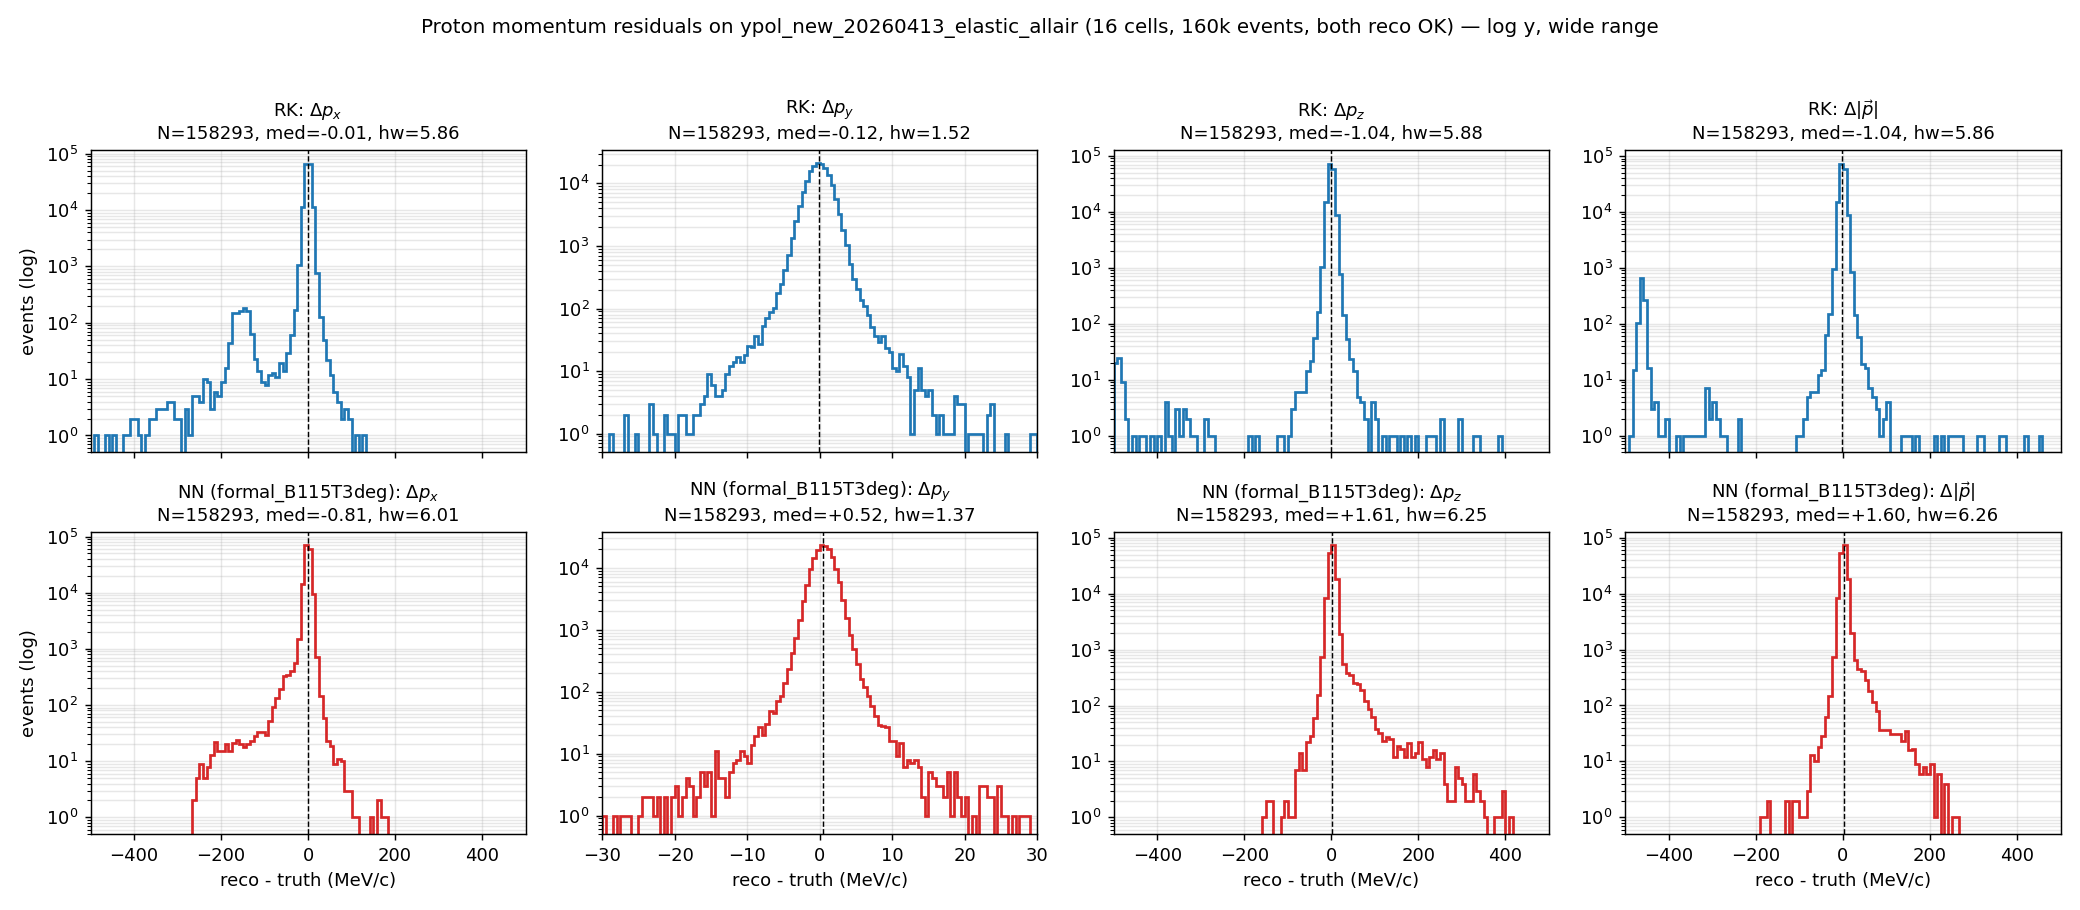
\includegraphics[width=\textwidth]{figures/ypol_phys_nn_vs_rk/residuals_grid_tail.png}
\caption{Reco $-$ truth 残差分布 (158\,293 事件 pool, log y, 宽 x). 上行: RK (蓝), 下行: NN (红). 列从左到右: $\Delta p_x$, $\Delta p_y$, $\Delta p_z$, $\Delta |\vec p|$. 黑虚线 = median, 标题给出 N、median、half-width. log y 用来暴露 RK 在 $\Delta p_x, \Delta p_z, \Delta|\vec p|$ 上量级达数百 MeV/$c$ 的灾难性失败模式.}
\end{figure}

\begin{figure}[H]
\centering
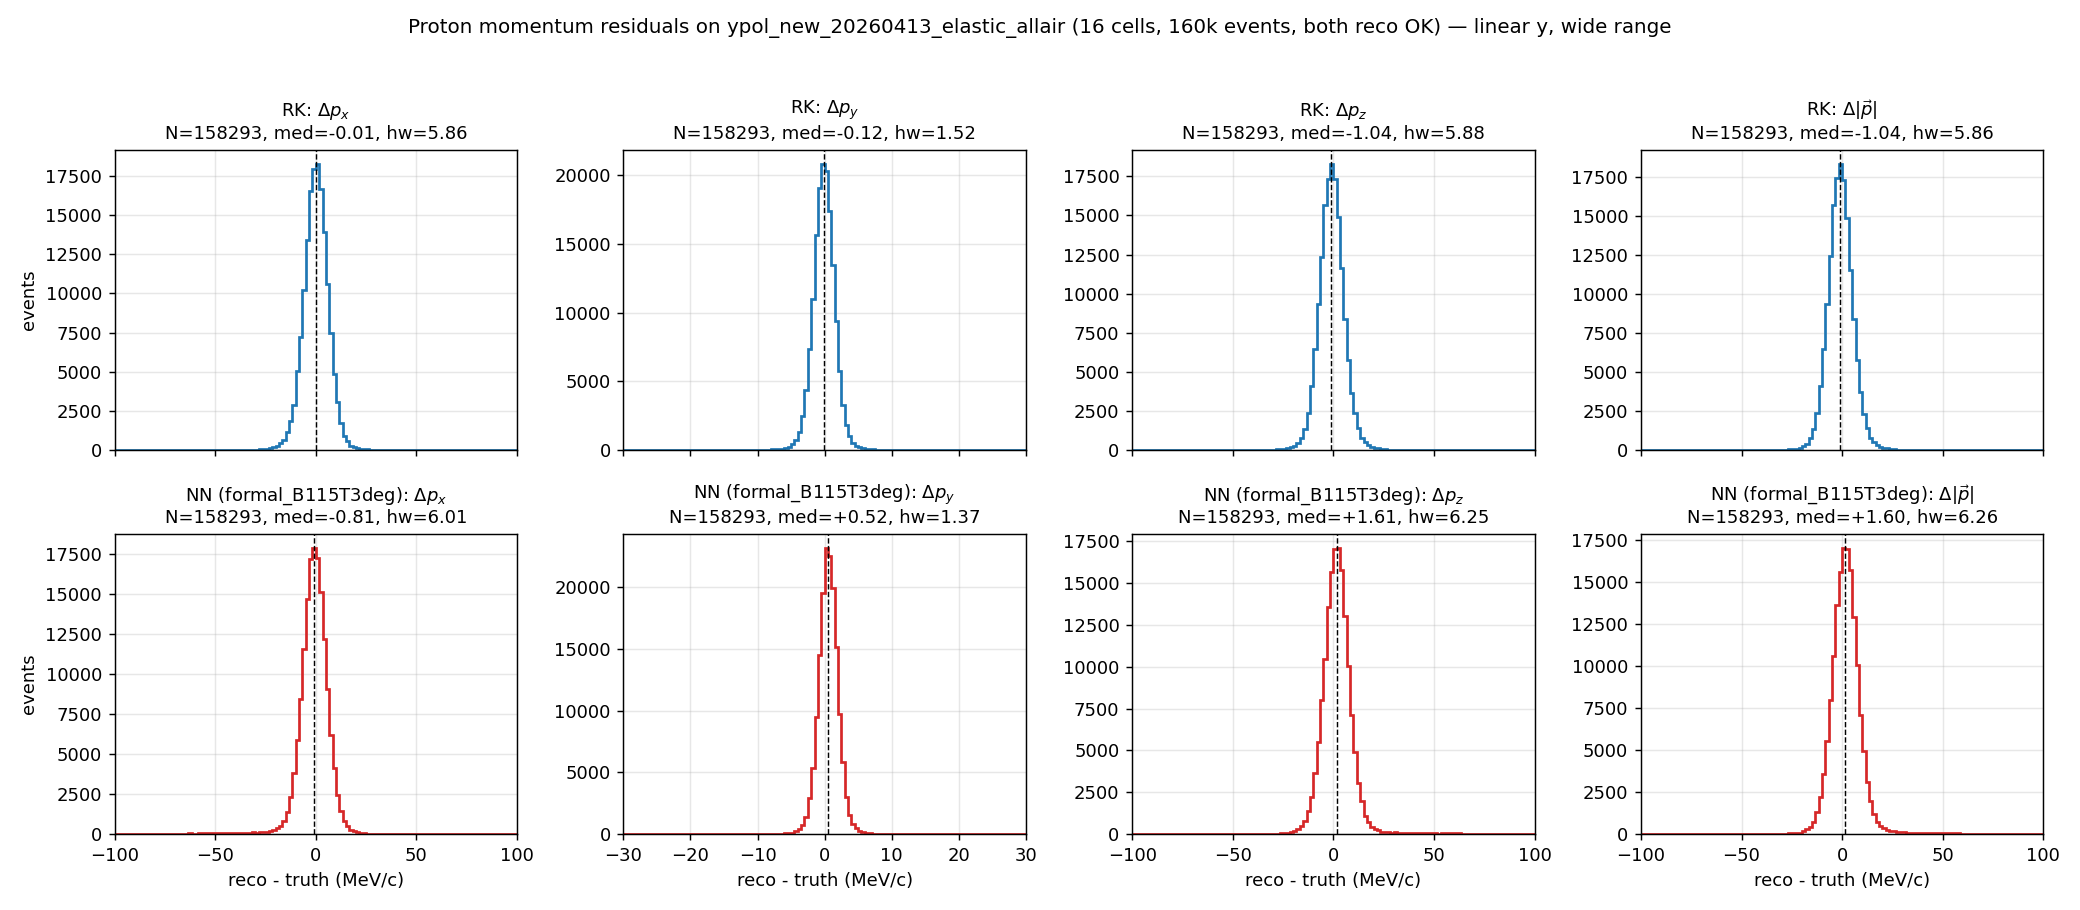
\includegraphics[width=\textwidth]{figures/ypol_phys_nn_vs_rk/residuals_grid_tail_linear.png}
\caption{同上, 但 y 轴取线性. 同样的 158\,293 事件 pool、同样的宽 x 范围. 线性 y 直观显示中央峰高度对比 (RK 与 NN 的中央峰高度量级一致), RK 的远尾在线性 y 下接近横轴, 而 log y 视图更适合定量比较尾部.}
\end{figure}

\begin{figure}[H]
\centering
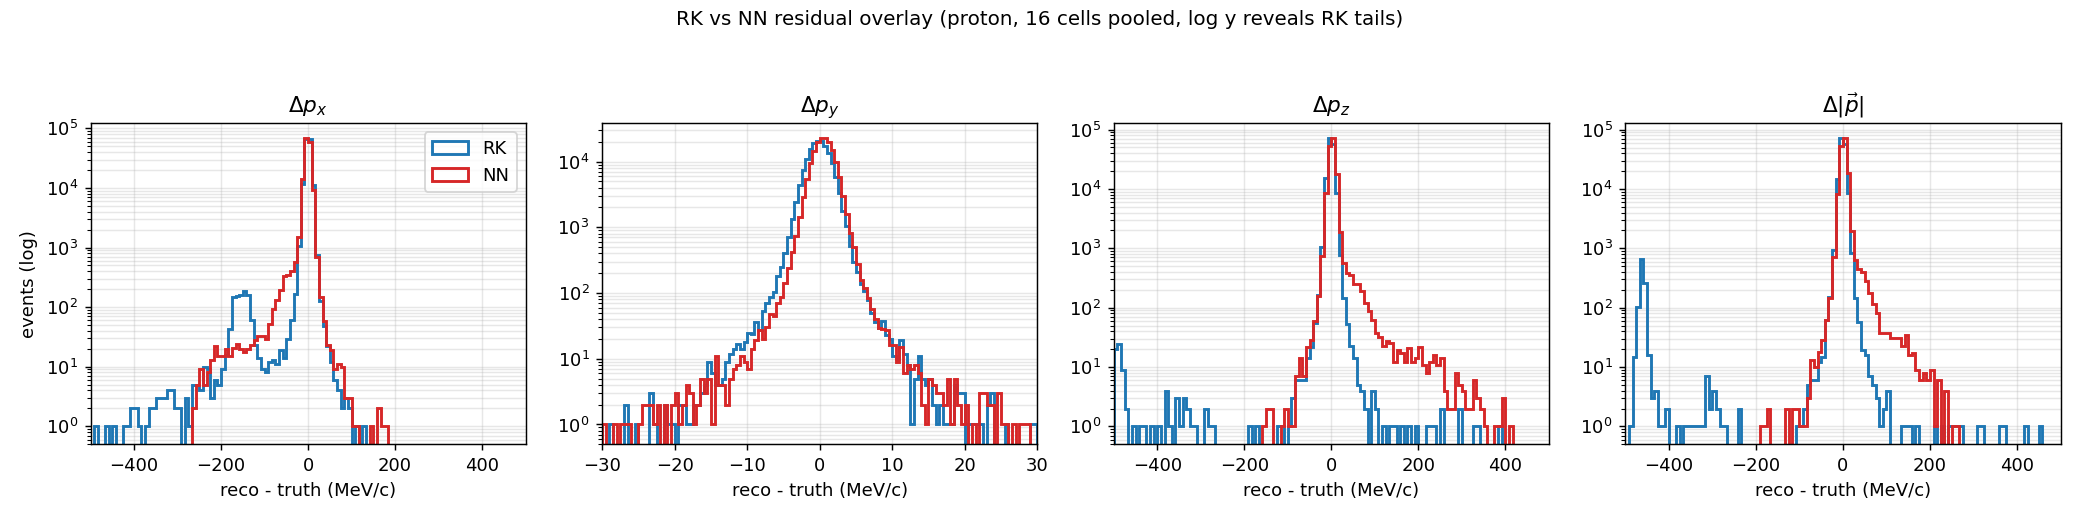
\includegraphics[width=\textwidth]{figures/ypol_phys_nn_vs_rk/residuals_overlay_tail.png}
\caption{RK (蓝) 与 NN (红) 残差在同一 panel 上叠加 (log y, 宽 x). 中央峰宽两者接近, 但 RK 的 $\Delta p_x, \Delta p_z, \Delta|\vec p|$ 在 $\pm 30$ MeV/$c$ 外仍可见明显的非高斯尾, 而 NN 没有.}
\end{figure}

\begin{figure}[H]
\centering
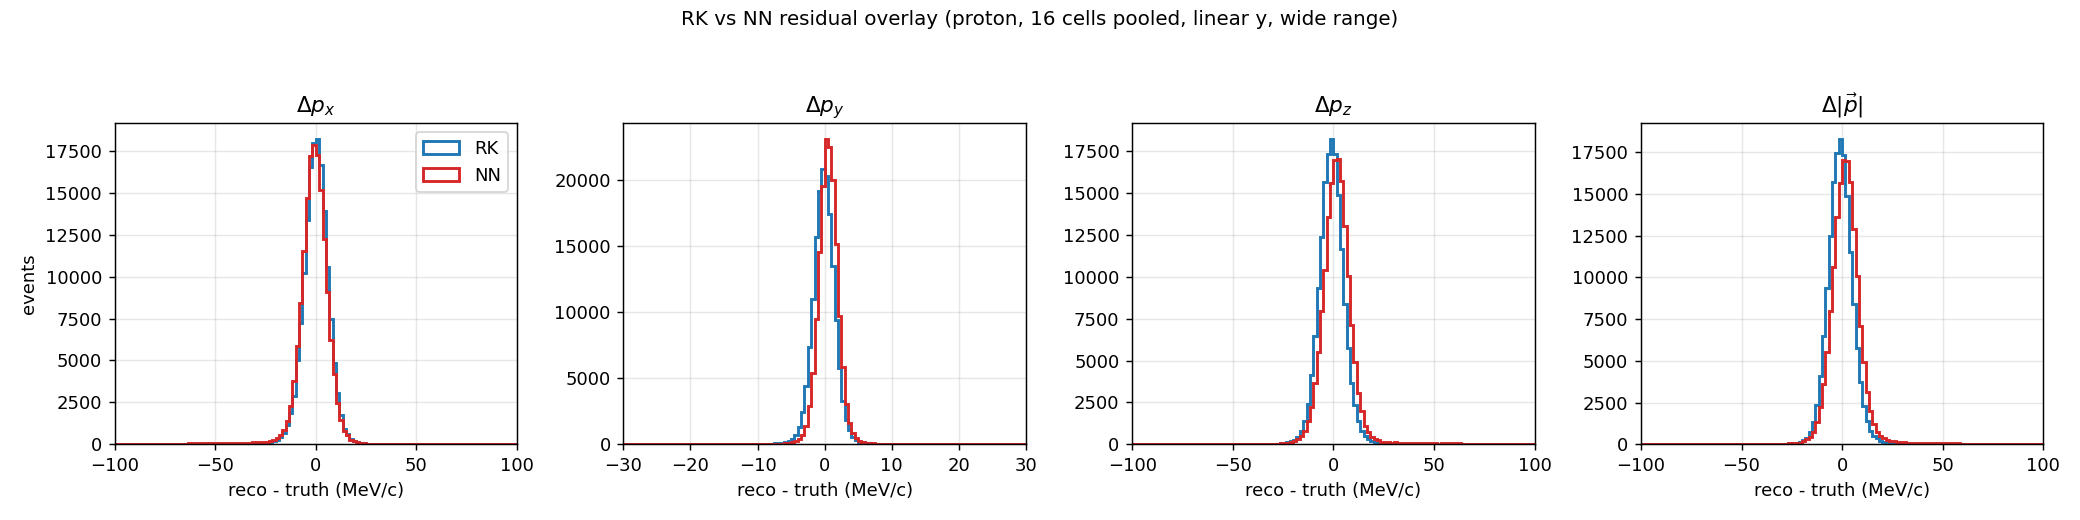
\includegraphics[width=\textwidth]{figures/ypol_phys_nn_vs_rk/residuals_overlay_tail_linear.png}
\caption{同上 overlay 视图但 y 轴线性. 中央峰高度对齐时 RK 与 NN 几乎完全重合, 尾部差异在线性 y 下不可见 —— 与上图的 log y 配合阅读.}
\end{figure}

\subsection{3.3 reco vs truth 二维对照}
\begin{figure}[H]
\centering
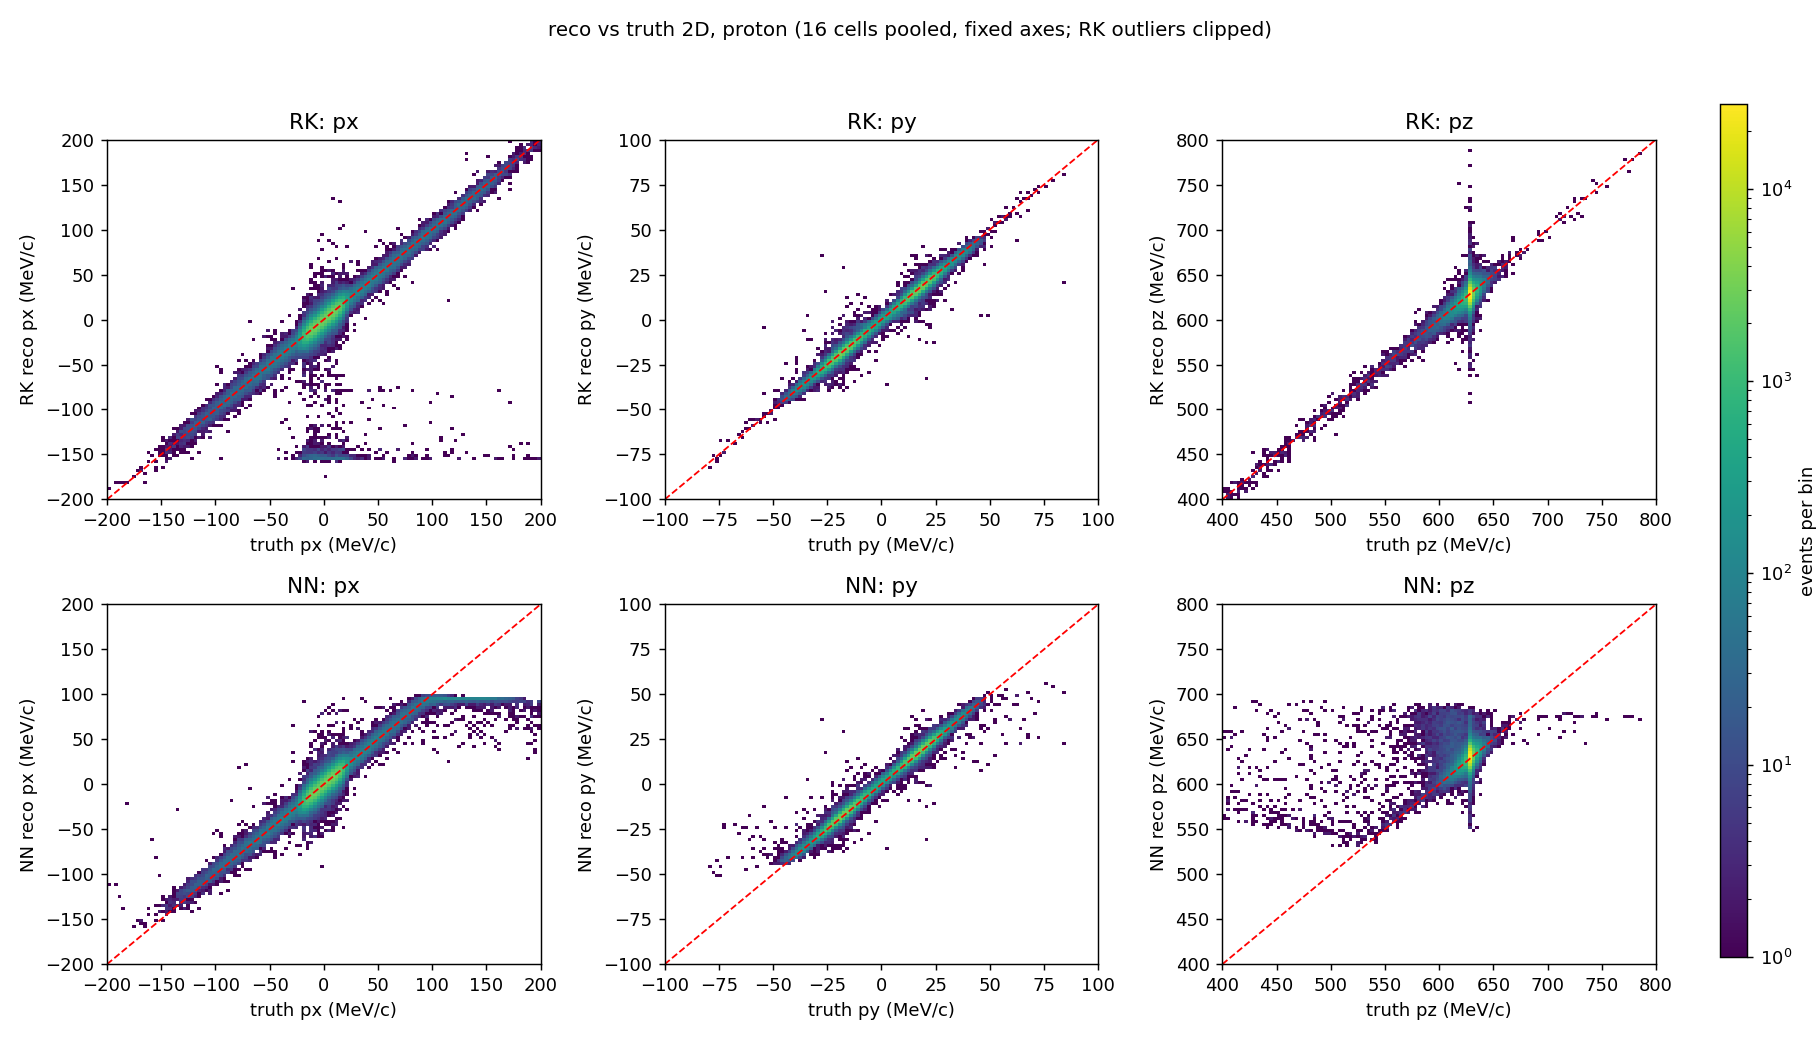
\includegraphics[width=0.95\textwidth]{figures/ypol_phys_nn_vs_rk/reco_vs_truth_2d.png}
\caption{reco vs truth 2D 直方图. 上行: RK; 下行: NN. 红虚线 $y = x$. 三列依次 $p_x, p_y, p_z$. 6 个 panel 共享同一 \texttt{LogNorm} 颜色映射, 右侧色标标出每 bin 的事件数 (events per bin, log 刻度). 两种方法在 $p_x, p_z$ 上都展现出物理上的对角线相关, NN 的对角线略宽但更对称, RK 在 $p_z$ 上有明显的离群点向下散开.}
\end{figure}

\section{4. 解读}

\subsection{4.1 中心宽度 (1$\sigma$): 两者基本相当, NN $p_y$ 反超}

NN 的 hidden-128/128/64 在 PDC$\to$target 这种近似线性几何映射上, 已经能达到 RK 解析重建的 1$\sigma$ 精度量级:
\begin{itemize}[nosep]
    \item $\Delta p_x$: RK 5.86 vs NN 6.01 (NN +2.6\%), 差距非常小.
    \item $\Delta p_y$: RK 1.52 vs NN \textbf{1.37} (NN $-9.9\%$, NN 反而更窄). 物理上 $p_y$ 不需解 dipole, 训练数据足够覆盖, NN 能学到的映射比 RK 用的简单两点斜率多一点上下文 (隐式利用了两层 PDC 的相关性).
    \item $\Delta p_z$: RK 5.88 vs NN 6.25 (NN +6.3\%).
\end{itemize}

\subsection{4.2 尾部: NN 显著优于 RK}

最戏剧的差异是 RMSE / 中心宽度比:
\[
    R_\text{tail} \equiv \text{RMSE}\,/\,(\sigma_\text{eff}=\text{half-width})
\]
理想高斯 $R_\text{tail} = 1$. 实测:
\begin{table}[H]
\centering\footnotesize
\begin{tabular}{lcc}
\toprule
量          & RK $R_\text{tail}$ & NN $R_\text{tail}$ \\
\midrule
$\Delta p_x$    & 17.08 / 5.86 = 2.92 & 11.73 / 6.01 = 1.95 \\
$\Delta p_y$    &  1.88 / 1.52 = 1.24 &  1.82 / 1.37 = 1.33 \\
$\Delta p_z$    & 46.36 / 5.88 = 7.88 & 13.43 / 6.25 = 2.15 \\
$\Delta|\vec p|$& 39.91 / 5.86 = 6.81 & 10.77 / 6.26 = 1.72 \\
\bottomrule
\end{tabular}
\end{table}

RK 的 $\Delta p_z, \Delta|\vec p|$ 在 RMSE 与 1$\sigma$ 之间相差近 \textbf{8 倍} —— 即\textbf{有少量事件残差量级达数百 MeV/$c$}。
这与 RK 报告 §1.3 / \texttt{rk\_reconstruction\_status\_20260416\_zh} 关于 dE/dx + $(u, v, p)$ 线性化在低 $|\vec p|$ 或大角度时失效的诊断一致.
NN 则不存在这种"灾难性失败"模式: 在训练分布内, 输出始终保持在 truth 附近 $\pm$几十 MeV/$c$.

\subsection{4.3 系统偏置 (median bias)}

\begin{itemize}[nosep]
    \item RK $\Delta p_x \approx 0$, $\Delta p_z = -1.04$ MeV/$c$ —— 1 MeV/$c$ 量级的负偏来自 dE/dx 模型对靶后到 PDC 段能损的轻微低估 (RK 报告 §1.3 已记录).
    \item NN $\Delta p_x = -0.81$, $\Delta p_y = +0.52$, $\Delta p_z = +1.61$ MeV/$c$ —— NN 全 3 方向\textbf{都} 有 $\sim$1 MeV/$c$ 系统偏. 这是训练损失 (无 bias 正则的纯 MSE) + 训练数据 z-score 中心 (训练样本与 elastic 样本的 PDC 击中分布不完全重合) 共同造成的, 数值与训练自检的 val bias 同量级.
\end{itemize}

\subsection{4.4 $\Delta p_y$ 为何 NN 比 RK 更窄}
RK 的 $p_y$ 来自 PDC1, PDC2 两层 y-strip 的两点斜率, 单层 $\sim 200\,\mu$m, 杠杆 $\sim 1.65$ m → 角度 $\sigma \approx 200\,\mu\text{m}/1.65\text{m} \approx 0.12$ mrad → $\sigma(p_y) \approx 627 \times 0.12 \times 10^{-3} \approx 0.08$ MeV/$c$ (量级估算, 多次散射贡献使其放大到 1.5 MeV/$c$ 量级).
NN 的输入是\textbf{两层 PDC 的全部 6 个坐标}, 包含 $p_y$ 对 $(x, z)$ 的弱关联 (磁场 fringing 在 y 上的二阶项), 学到了一个比纯两点斜率略优的统计 estimator —— 因此 1$\sigma$ 略小, 代价是引入一个无害的 $+0.5$ MeV/$c$ bias.

\section{5. 适用边界与下一步}

\subsection*{5.1 适用边界}
\begin{itemize}[nosep]
    \item \textbf{适用}: ypol elastic 类样本 ($p_z\sim 627$, $p_T\lesssim 100$ MeV/$c$), 几何固定为 \texttt{geometry\_B115T\_pdcOptimized\_20260227\_target3deg.mac}.
    \item \textbf{需谨慎}: QMD breakup / 大 $p_T$ 事件 (训练域只到 100 MeV/$c$). 本样本里 $p_T > 100$ 的 2.9\% 事件 NN 性能未验证.
    \item \textbf{域漂移}: 不同几何 macro / 不同 PDC 噪声 $\sigma$ / 不同磁场设置都可能导致输入 z-score 失配. 已有的 \texttt{run\_domain\_matched\_retrain.sh} 是为 z\_pol/y\_pol 域匹配再训练设计, 但当前次模型 (\texttt{20260228\_002757}) 仅用了 44 train rows, 误差 RMSE > 100 MeV/$c$, 不可用; 域匹配再训练需要重新跑足量数据.
\end{itemize}

\subsection*{5.2 推荐使用方式}
基于本评估, 在 ypol elastic 类分析里 NN 重建 \textbf{可以直接替代 RK}, 收益:
\begin{itemize}[nosep]
    \item 通过率提到 100\% (RK 损失 $\sim$1.1\% 事件);
    \item 消除 RK 的灾难性 $|\vec p|$ 失败 (RMSE 减少 $\sim 4\times$);
    \item $p_y$ 1$\sigma$ 略优.
\end{itemize}
代价:
\begin{itemize}[nosep]
    \item 引入 1\textendash 2 MeV/$c$ 量级的 3 方向 bias (低于本样本中 $|\vec p|$ 的 0.3\%, 对反应平面 / R 比值类分析量级可忽略).
    \item 没有 RK 的 $\chi^2$ / Laplace 误差估计输出, 不便做 per-event 精度加权.
\end{itemize}

\subsection*{5.3 下一步建议 (按优先级)}
\begin{enumerate}[nosep]
    \item 把同一 NN 推理跑到 \texttt{eval\_target3deg\_smoke\_20260228\_ypol} / \texttt{eval\_20260227\_235751} 上, 看 $\Delta R_x^\text{rot}$ 受 NN 系统偏的影响 (预计 $<1\%$).
    \item 训练一份 $R = 200$ disk + $p_z\in[400, 800]$ 的"大窗"模型, 覆盖 QMD breakup; 重新评估在 ypol elastic 上是否回退.
    \item 在 NN 输出旁加一个解析的 per-event uncertainty head (heteroscedastic loss), 以便后续 $\chi^2$ 加权.
\end{enumerate}

\section*{Artifacts}
\begin{itemize}[nosep]
    \item NN reco 输出: \texttt{build/test\_output/ypol\_phys\_20260428/reco\_nn/<tag>\_reco\_nn.root}
    \item 抽取脚本: \texttt{scripts/analysis/ypol\_phys/extract\_proton\_rk\_nn.C}
    \item 残差分析脚本: \texttt{scripts/analysis/ypol\_phys/analyze\_nn\_vs\_rk\_residuals.py}
    \item Per-cell CSV: \texttt{build/test\_output/ypol\_phys\_20260428/csv\_rk\_nn/}
    \item 残差汇总: \texttt{docs/reports/reconstruction/momentum\_reco/nn/figures/ypol\_phys\_nn\_vs\_rk/summary.\{json,txt\}}
    \item Per-cell 表: 同目录 \texttt{per\_cell\_summary.csv}
\end{itemize}

\end{document}
